\documentclass[../main.tex]{subfiles}
\begin{document}

\section{6D Object Pose Estimation \\ \normalfont\normalsize\texttt{Mathias Emil Slettemark-Nielsen}} \label{sec:pose_estimation}

Since the previous sections assume that the pose of the obstacles are known, it is relevant to inspect methods that can be used to recognize and pose estimate a potential obstacle. In this section the dataset LINEMOD \cite{linemod} will be used to determine the performance of the pose estimating network iterative dense fusion and compared against a 3D-3D pose estimating method.

\subsection{The Dataset of Objects \\ \normalfont\normalsize\texttt{Mikkel Larsen}} \label{subsec:dataset}

Before delving into pose estimation a dataset is introduced. The dataset should contain variations in scale, viewpoint and illumination. Furthermore, the dataset should contain cluttered scenes and occlusion of objects.

The dataset used in this report is the LINEMOD dataset and can be found here \cite{linemod_dataset}. The LINEMOD dataset consists of $13$ objects which is shown in figure \ref{fig:linemod_objects}. The dataset contains a 3D model of each object, the maximum diameter of each object, the color images, the aligned depth images and the ground truth mask, rotation and translation.

\begin{figure}[H]
    \centering
    \begin{subfigure}[t]{0.19\textwidth}
        \centering
        \captionsetup{width=.9\textwidth}
        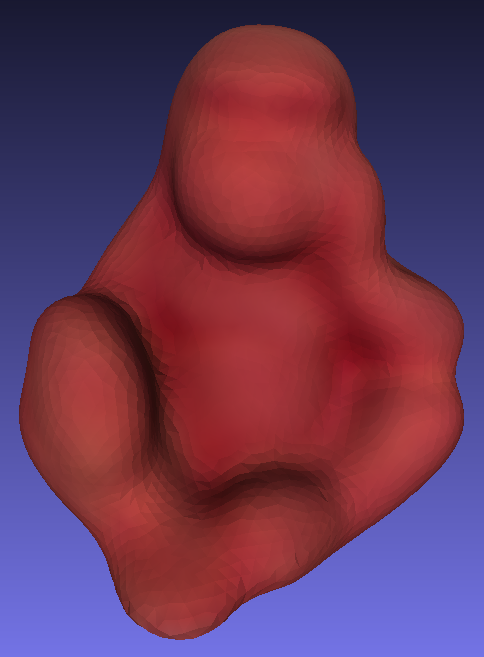
\includegraphics[width=0.9\textwidth, height=20mm, keepaspectratio]{figures/linemod/ape_obj01.png}
        \caption{Ape}
        \label{subfig:obj_ape}
    \end{subfigure}
    \begin{subfigure}[t]{0.19\textwidth}
        \centering
        \captionsetup{width=.9\textwidth}
        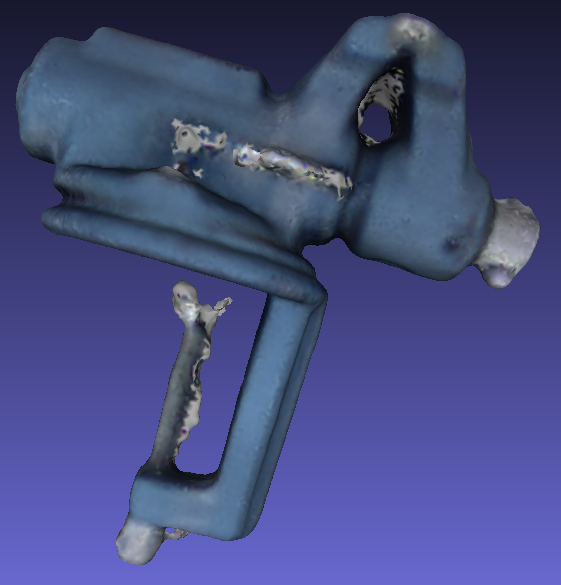
\includegraphics[width=0.9\textwidth, height=20mm, keepaspectratio]{figures/linemod/bench_vi_obj02.png}
        \caption{Bench vise}
        \label{subfig:obj_bench_vi}
    \end{subfigure}
    \begin{subfigure}[t]{0.19\textwidth}
        \centering
        \captionsetup{width=.9\textwidth}
        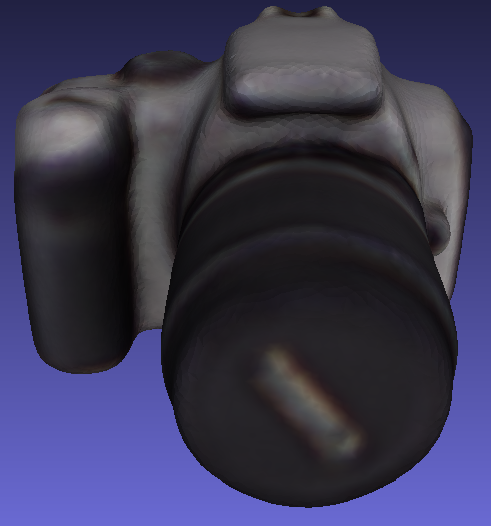
\includegraphics[width=0.9\textwidth, height=20mm, keepaspectratio]{figures/linemod/camera_obj04.png}
        \caption{Camera}
        \label{subfig:obj_camera}
    \end{subfigure}
    \begin{subfigure}[t]{0.19\textwidth}
        \centering
        \captionsetup{width=.9\textwidth}
        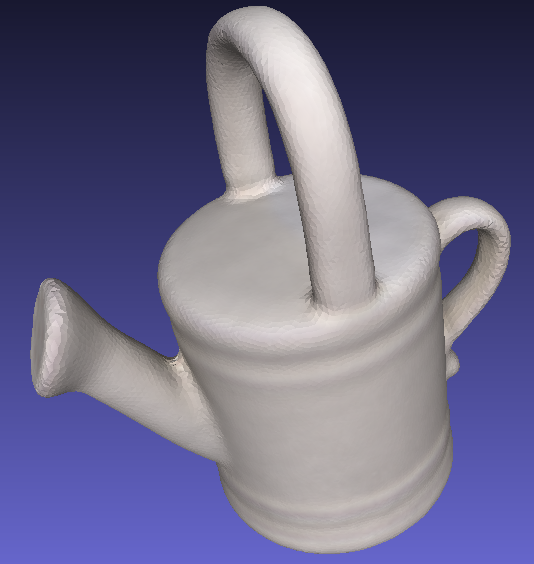
\includegraphics[width=0.9\textwidth, height=20mm, keepaspectratio]{figures/linemod/can_obj05.png}
        \caption{Can}
        \label{subfig:obj_can}
    \end{subfigure}
    \begin{subfigure}[t]{0.19\textwidth}
        \centering
        \captionsetup{width=.9\textwidth}
        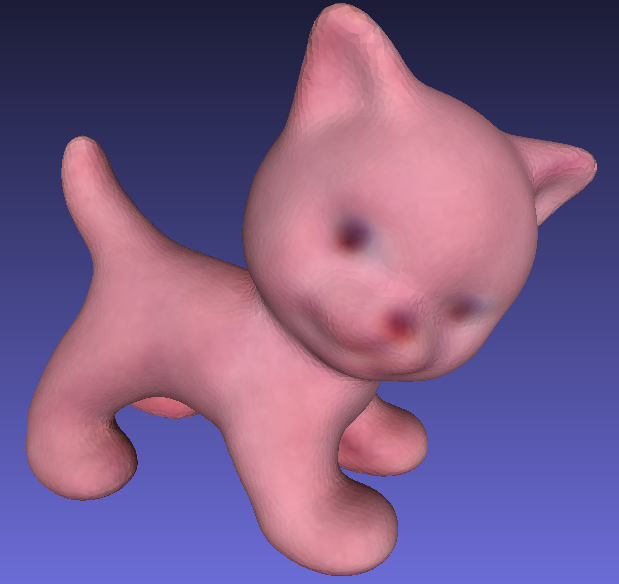
\includegraphics[width=0.9\textwidth, height=20mm, keepaspectratio]{figures/linemod/cat_obj06.png}
        \caption{Cat}
        \label{subfig:obj_cat}
    \end{subfigure}
    \begin{subfigure}[t]{0.19\textwidth}
        \centering
        \captionsetup{width=.9\textwidth}
        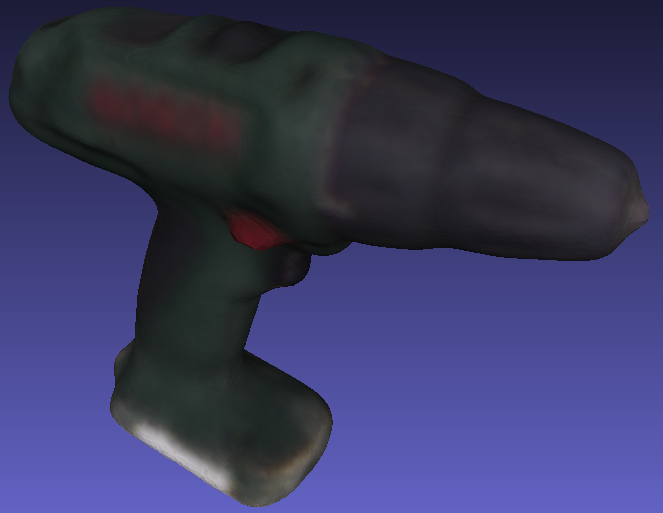
\includegraphics[width=0.9\textwidth, height=20mm, keepaspectratio]{figures/linemod/drill_obj08.png}
        \caption{Drill}
        \label{subfig:obj_drill}
    \end{subfigure}
    \begin{subfigure}[t]{0.19\textwidth}
        \centering
        \captionsetup{width=.9\textwidth}
        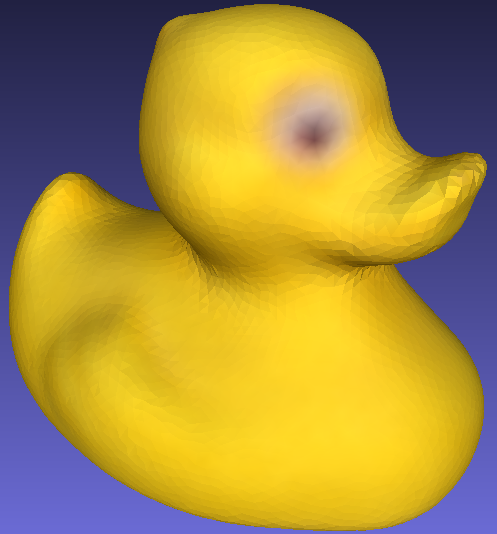
\includegraphics[width=0.9\textwidth, height=20mm, keepaspectratio]{figures/linemod/duck_obj09.png}
        \caption{Duck}
        \label{subfig:obj_duck}
    \end{subfigure}
    \begin{subfigure}[t]{0.19\textwidth}
        \centering
        \captionsetup{width=.9\textwidth}
        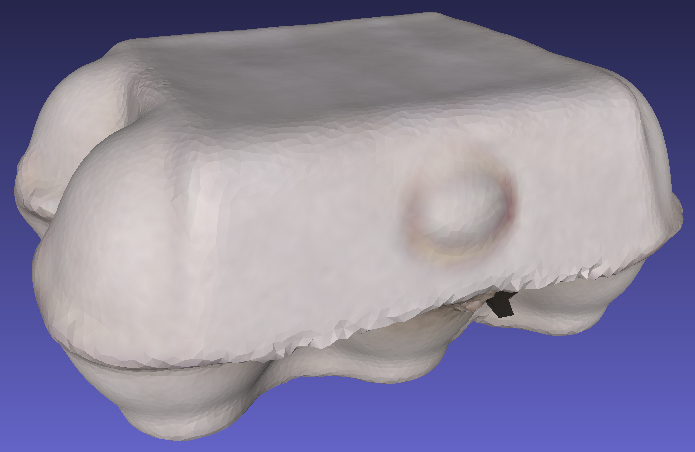
\includegraphics[width=0.9\textwidth, height=20mm, keepaspectratio]{figures/linemod/eggbox_obj10.png}
        \caption{Egg box}
        \label{subfig:obj_eggbox}
    \end{subfigure}
    \begin{subfigure}[t]{0.19\textwidth}
        \centering
        \captionsetup{width=.9\textwidth}
        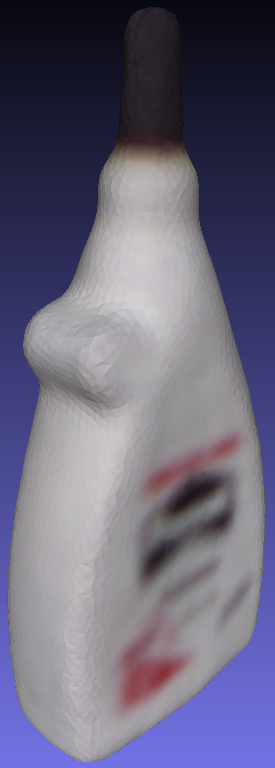
\includegraphics[width=0.9\textwidth, height=20mm, keepaspectratio]{figures/linemod/glue_obj11.png}
        \caption{Glue}
        \label{subfig:obj_glue}
    \end{subfigure}
    \begin{subfigure}[t]{0.19\textwidth}
        \centering
        \captionsetup{width=.9\textwidth}
        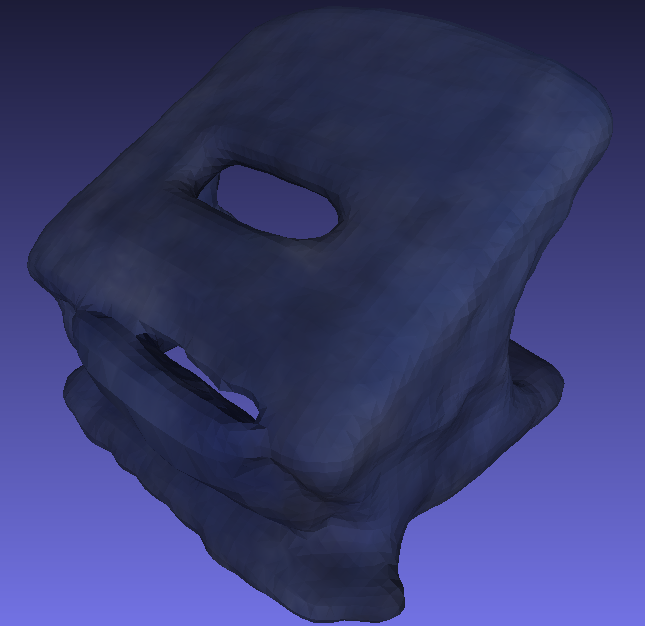
\includegraphics[width=0.9\textwidth, height=20mm, keepaspectratio]{figures/linemod/hole_p_obj12.png}
        \caption{Hole puncher}
        \label{subfig:obj_hole_p}
    \end{subfigure}
    \begin{subfigure}[t]{0.19\textwidth}
        \centering
        \captionsetup{width=.9\textwidth}
        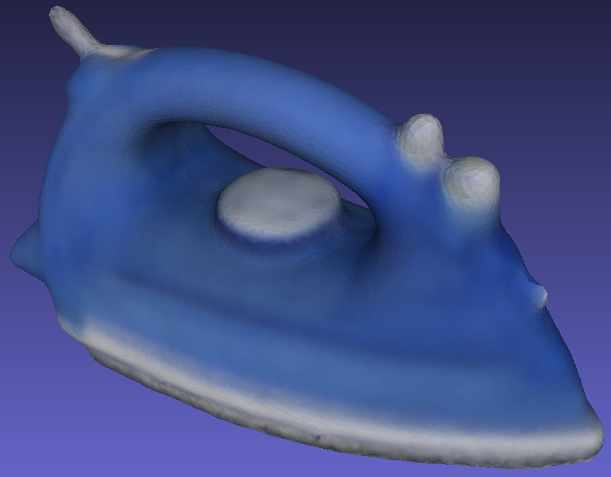
\includegraphics[width=0.9\textwidth, height=20mm, keepaspectratio]{figures/linemod/iron_obj13.png}
        \caption{Iron}
        \label{subfig:obj_iron}
    \end{subfigure}
    \begin{subfigure}[t]{0.19\textwidth}
        \centering
        \captionsetup{width=.9\textwidth}
        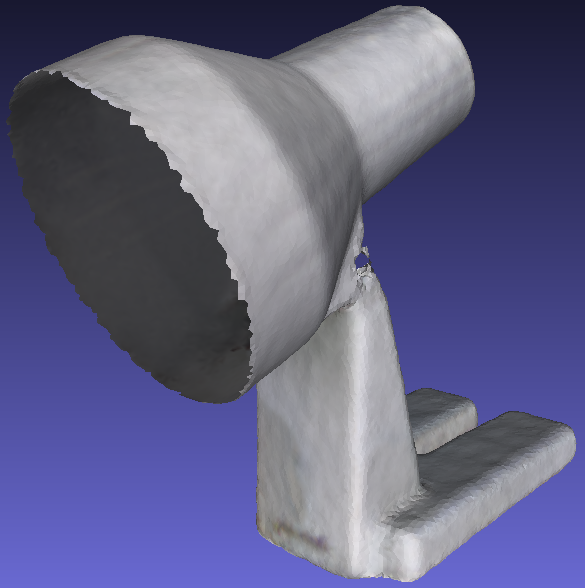
\includegraphics[width=0.9\textwidth, height=20mm, keepaspectratio]{figures/linemod/lamp_obj14.png}
        \caption{Lamp}
        \label{subfig:obj_lamp}
    \end{subfigure}
    \begin{subfigure}[t]{0.19\textwidth}
        \centering
        \captionsetup{width=.9\textwidth}
        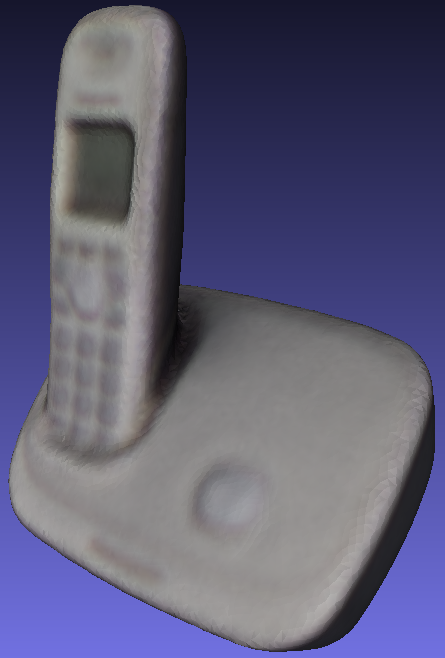
\includegraphics[width=0.9\textwidth, height=20mm, keepaspectratio]{figures/linemod/phone_obj15.png}
        \caption{Phone}
        \label{subfig:obj_phone}
    \end{subfigure}
    \caption{Illustrations of the objects from the LINEMOD dataset.}
    \label{fig:linemod_objects}
\end{figure}

Examples of the data from the LINEMOD dataset are shown in figure \ref{fig:linemod_examples}. The examples illustrates the variantions in scale, viewpoint and illumination. Moreover, the cluttered scenes and the occlusion of objects can be seen. 

\begin{figure}[H]
    \centering
    \begin{subfigure}[t]{0.24\textwidth}
        \centering
        \captionsetup{width=.9\textwidth}
        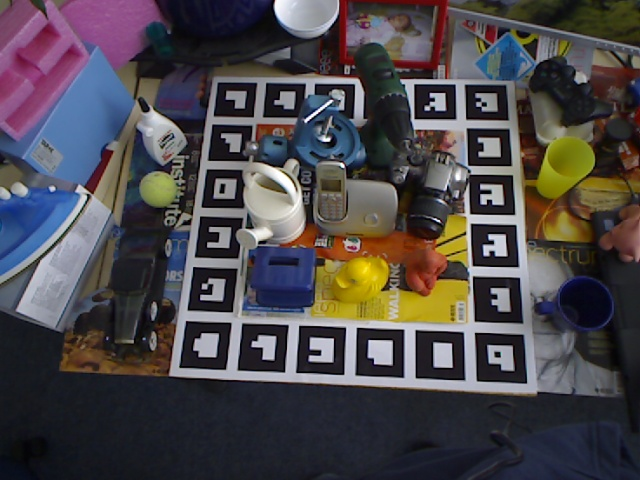
\includegraphics[width=0.9\textwidth]{figures/linemod/example01.png}
        % \caption{}
        \label{subfig:linemod_example01}
    \end{subfigure}
    \begin{subfigure}[t]{0.24\textwidth}
        \centering
        \captionsetup{width=.9\textwidth}
        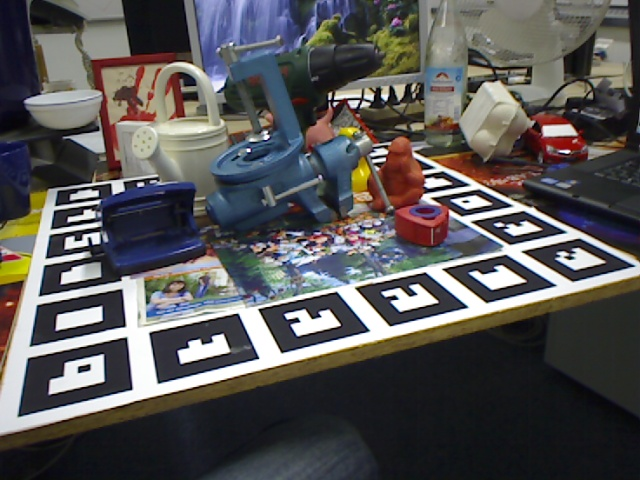
\includegraphics[width=0.9\textwidth]{figures/linemod/example02.png}
        % \caption{}
        \label{subfig:linemod_example02}
    \end{subfigure}
    \begin{subfigure}[t]{0.24\textwidth}
        \centering
        \captionsetup{width=.9\textwidth}
        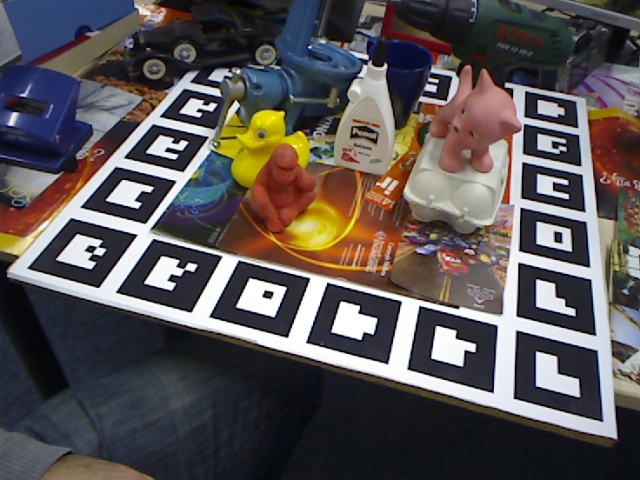
\includegraphics[width=0.9\textwidth]{figures/linemod/example03.png}
        % \caption{}
        \label{subfig:linemod_example03}
    \end{subfigure}
    \begin{subfigure}[t]{0.24\textwidth}
        \centering
        \captionsetup{width=.9\textwidth}
        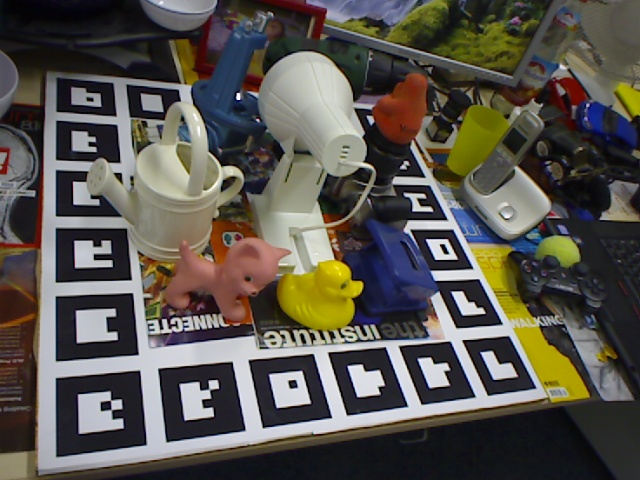
\includegraphics[width=0.9\textwidth]{figures/linemod/example04.png}
        % \caption{}
        \label{subfig:linemod_example04}
    \end{subfigure}
    \caption{Examples of data from the LINEMOD dataset.}
    \label{fig:linemod_examples}
\end{figure}

The LINEMOD dataset consist of $1236$ ape images, $1215$ bench vise images, $1201$ camera images, $1196$ can images, $1179$ cat images, $1188$ drill images, $1254$ duck images, $1253$ egg box images, $1220$ glue images, $1237$ hole puncher images, $1152$ iron images, $1227$ lamp images and $1225$ phone images. Thus, a total of $15783$ images.

To evaluate pose estimations the matching scores ADD, for non-symmetric object, and ADD-S, for symmetric objects are used, which is introduced in \cite{linemod_matching_score}. The symmetric objects are the egg box shown in figure \ref{subfig:obj_eggbox} and the glue shown in figure \ref{subfig:obj_glue}. The average ADD matching score for a 3D model $\mathcal{M}$ is computed as
\begin{equation}
    \text{ADD score} = \avg_{x \in \mathcal{M}} \big \| (R x + T) - (\tilde{R} x + \tilde{T}) \big \|
    \label{eqn:linemod_add}
\end{equation}
where the ground truth is denoted $R$ for rotation and $T$ for translation, $\tilde{R}$ and $\tilde{T}$ are the estimated rotation and translation, respectively, and $x$ is the model points. The average ADD-S matching score is computed as
\begin{equation}
\text{ADD-S score} = \avg_{x_1 \in \mathcal{M}} \min_{x_2 \in \mathcal{M}} \| (R x_1 + T) - (\tilde{R} x_2 + \tilde{T}) \big \|
\label{eqn:linemod_add_s}
\end{equation}
where $x_2$ is closest point to $x_1$ within $\mathcal{M}$. 

To classify if a pose is correct compared to the ground truth pose, \autoref{eq:cor:pos:score} must be true, else is the estimated pose classified as a wrong pose.
\begin{equation}
    k_{m}\cdot d \geq m
    \label{eq:cor:pos:score}
\end{equation}

Where $k_{m}$ is a chosen constant which is set to $0.1$ and $d$ is the diameter of $\mathcal{M}$.

\subsection{Iterative Dense Fusion \\ \normalfont\normalsize\texttt{Mathias Emil Slettemark-Nielsen}} \label{subsec:dense_fusion}
To estimate a 6D object pose the method Iterative Dense Fusion, DenseFusion, is implemented. DenseFusion is introduced in \cite{densefusion} and uses deep networks for pose estimation from RBG-D inputs. Figure \ref{fig:dense_fusion_overview} illustrates an overview of DenseFusion.

\begin{figure}[H]
    \centering
    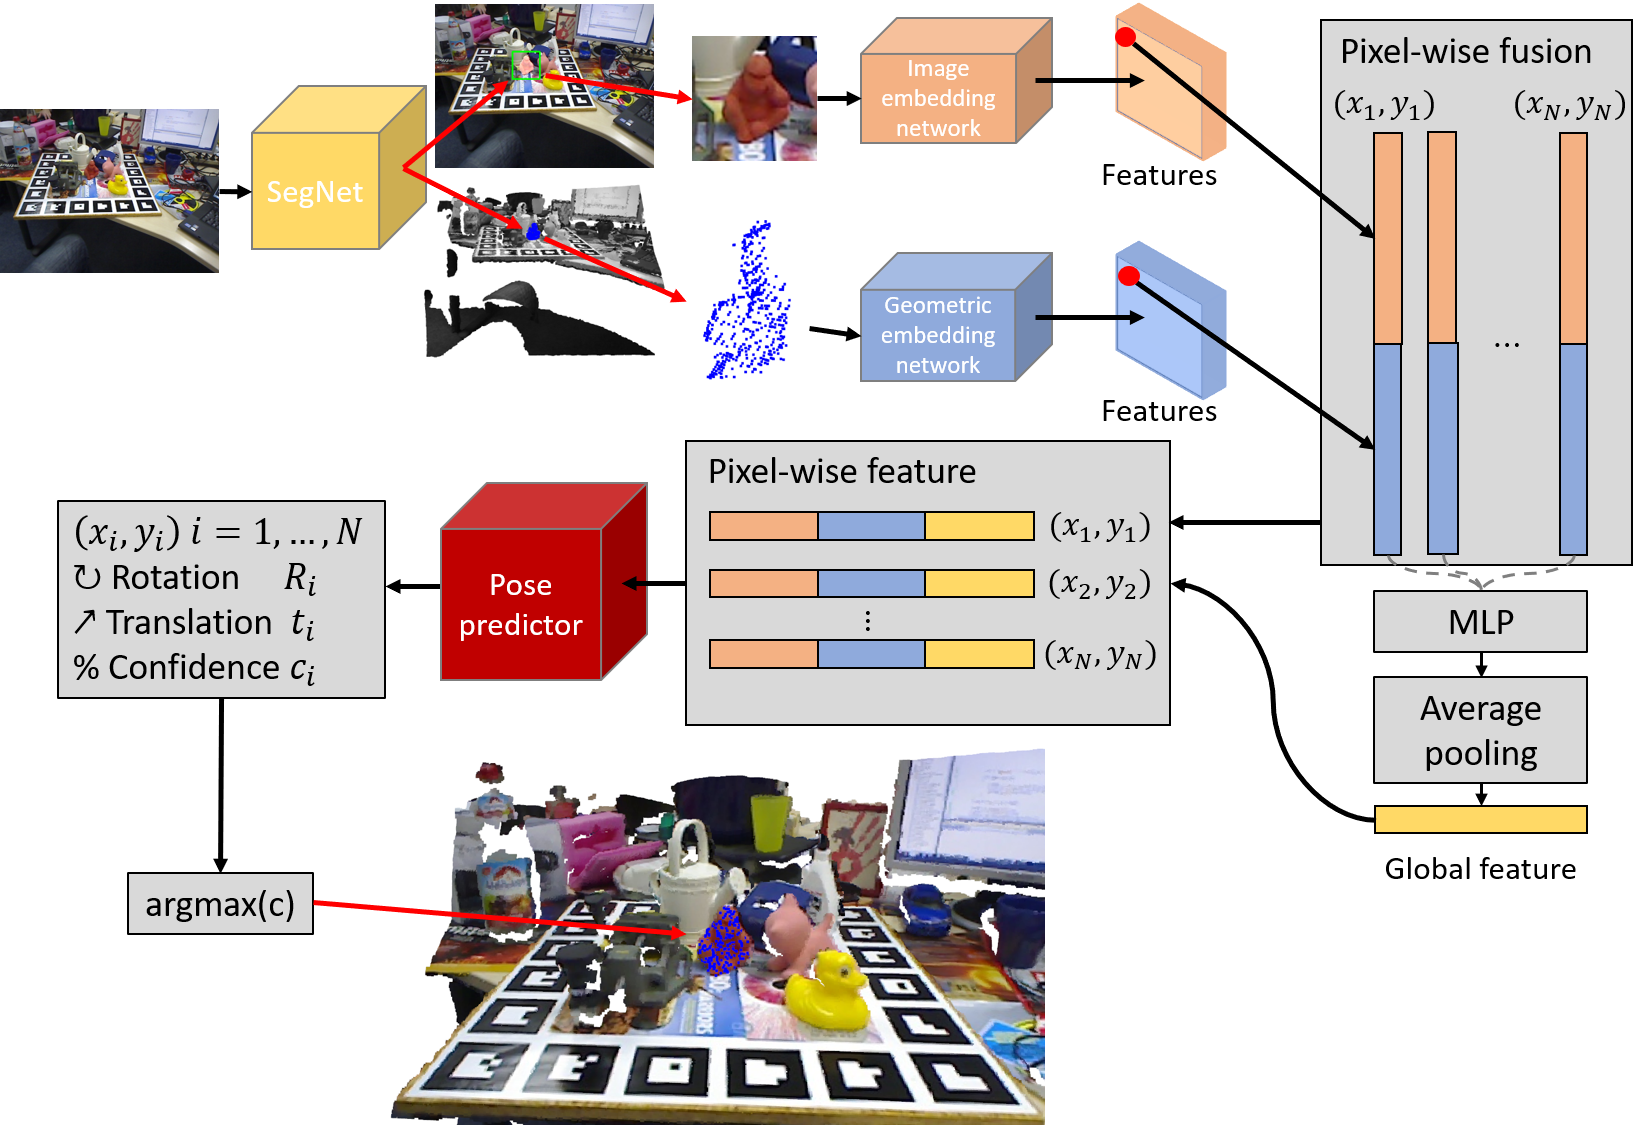
\includegraphics[width=\textwidth]{figures/dense_fusion/dense_fusion_overview.png}
    \caption{An illustration of the 6D pose estimation method DenseFusion, where the object of interest is found in the RGB-D input. The RGB-D input is then cropped and the RGB and D input is fed through different networks, thus creating color and point features. The features are fused with a global featue, and a network predicts a pose for each feature. The pose with the highest confidence score is the final 6D pose estimation.}
    \label{fig:dense_fusion_overview}
\end{figure}

DenseFusion consist of five stages:
\begin{enumerate}
    \item A deep network that performs semantic segmentation, i.e. linking each pixel to a class label. The found mask of the object is used to create a point cloud of the object and a cropped color image.
    \item A fully convolutional network that processes the color information and maps each pixel in the cropped image to a color feature vector, thus creating a feature map.
    \item A PointNet-based \cite{pointnet} network that processes each point in the masked 3D point cloud to a geometric feature vector, thus creating a feature cloud.
    \item A pixel-wise fusion network that combines color feature and geometric feature with a global feature, and outputs a estimation of the 6D pose for each fusion. A confidence is estimated for each fusion to pick the final pose.
    \item A network to improve the predicted pose by estimating a residual pose. 
\end{enumerate}

\subsubsection{Semantic Segmentation\\ \normalfont\normalsize\texttt{Mathias Emil Slettemark-Nielsen}} \label{subsubsec:segnet}
To be able to estimate the pose of an object, the object must first be identified in the image. This is done by the use of the deep network SegNet \cite{segnet} which is created for semantic segmentation. Other alternatives such as U-Net \cite{unet} could also have been used for semantic segmentation. SegNet consist of an encoder network, a corresponding decoder network and a pixel-wise classification layer. The architecture of SegNet is illustrated in figure \ref{fig:segnet_architecture}.

\begin{figure}[H]
    \centering
    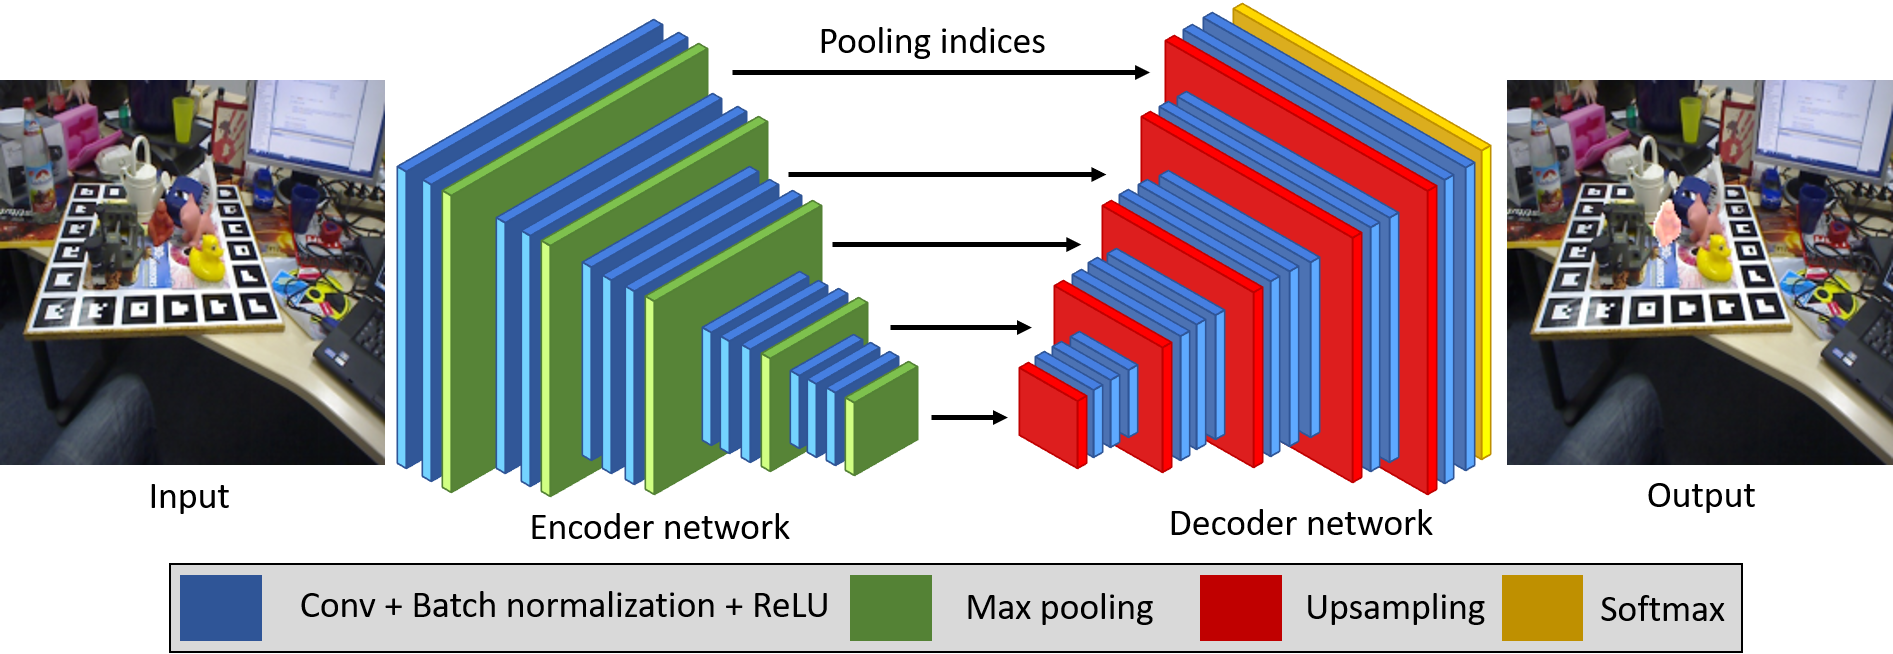
\includegraphics[width=\textwidth]{figures/segmentation/segnet_architecture.png}
    \caption{An illustration of the SegNet architecture, where the input image is from the LINEMOD dataset, and the output is the input with the prediction added.}
    \label{fig:segnet_architecture}
\end{figure}

\textbf{Encoder network:} To find features in the input image the first $13$ convolutional layers in the VGG16 network \cite{vgg} is used. The encoder network consist of several encoders where each encoder performs convolution, batch normalization \cite{batch_norm} and Rectified Linear Unit, ReLU, \cite{relu}. After each encoder max pooling with a $(2 \times 2)$ window and a stride of $2$ is performed. The locations of the maximum feature value in each max pooling window, the pooling indices, is stored for each encoder feature map.

\textbf{Decoder network:} To upsample the feature map the decoder network consist of a hierarchy of decoders, one for each corresponding encoder. Each decoder uses the corresponding pooling indices to upsample the input feature map. This is illustrated in figure \ref{fig:segnet_upsampling_feature_map}, and it can be seen that a sparse feature map is produced. After each upsampling convolution, batch normalization and ReLU is performed on the feature map.

\begin{figure}[H]
    \centering
    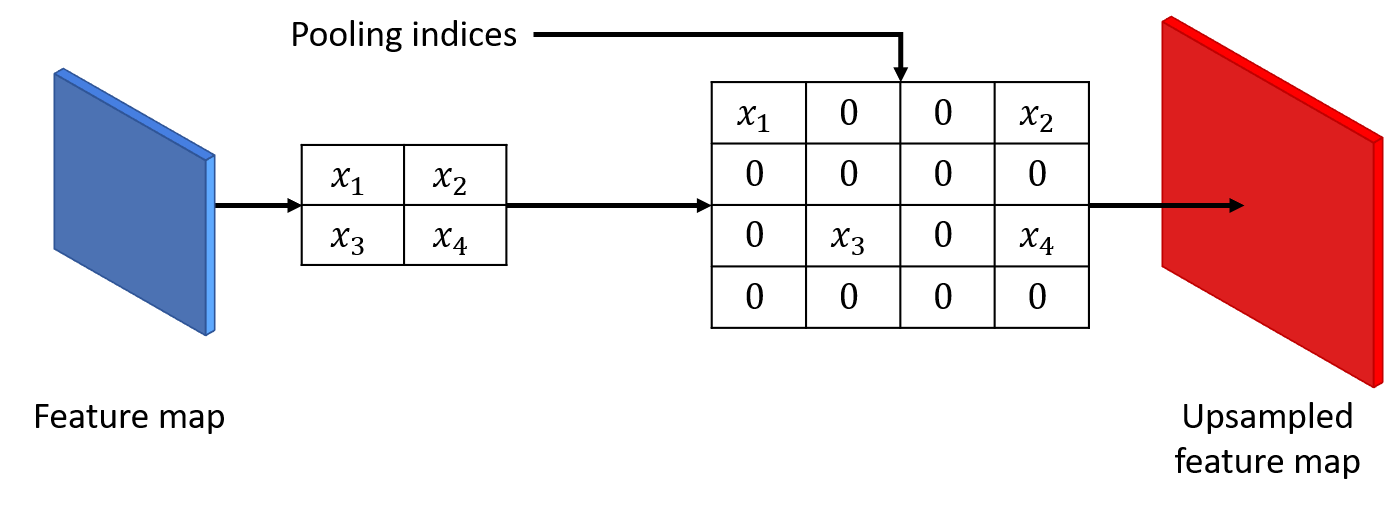
\includegraphics[width=0.75\textwidth]{figures/segmentation/segnet_upsampling_of_feat_map.png}
    \caption{An illustration of SegNet decoders where $x_1$, $x_2$, $x_3$ and $x_4$ correspond to values in a feature map. The pooling indices are used to upsample the feature map.}
    \label{fig:segnet_upsampling_feature_map}
\end{figure}

% Comparing SegNet to U-Net, U-Net does not reuse pooling indices but instead transfers the entire feature map to the corresponding decoders and concatenates them to a upsampled decoder feature map.

\textbf{Pixel-wise classification:} The final feature map is fed to a softmax classifier \cite{softmax}, that classifies each pixel independently. The output of the softmax classifier is a image of probabilities with as many channels as number of classes, e.g. background and ape.

\textbf{Implementation:} The LINEMOD dataset provides masks with one object, thus a SegNet model has to be trained for each object. The following models from figure \ref{fig:linemod_objects} are implemented: ape, bench vise, camera, cat and duck. The dataset is split into approximately $15\ \%$ training and $85\ \%$ testing, where the training is repeated for $20$ iteration and then the model is tested on the testing set.

The training set is artificially enlarged by the use of data augmentation, where rotation and color jitter is applied. For rotation augmentation the data is either flipped left to right, up to down or left to right followed by up to down. For color augmentation the data is jittered in brightness, contrast, saturation and hue.

The Adam optimizer \cite{adam} is used with a learning rate of $0.0001$, coefficients for computing running average of gradient $\beta_1 = 0.9$ and its square $\beta_2 = 0.999$ and the term added to the denominator to improve numerical stability $\epsilon = 10^{-8}$.

\textbf{Evaluation:} To evaluate the trained SegNet model the SegNet results from \cite{posecnn} are used which can be found here \cite{linemod_preprocessed}. For evaluation of object detection the metric Intersection over Union, IoU, is used and is illustrated in figure \ref{fig:iou_calculation}.

\begin{figure}[H]
    \centering
    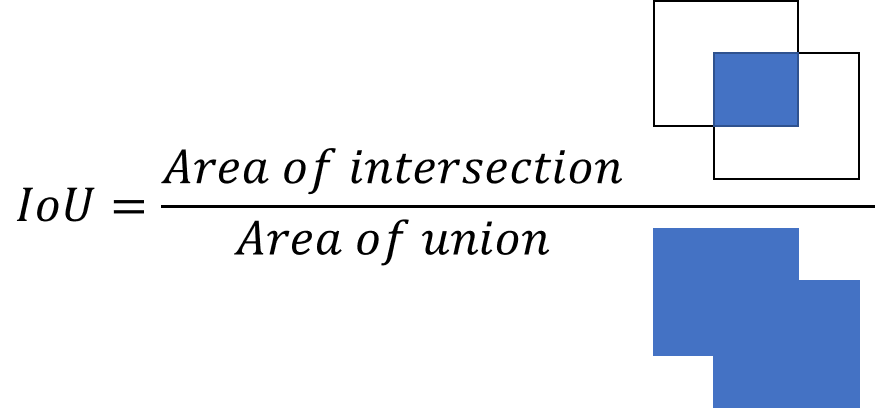
\includegraphics[width=0.5\textwidth]{figures/segmentation/iou.png}
    \caption{An illustration of Intersection over Union, IoU. The intersection is the overlap of the prediction and ground truth, and the union is the combined area.}
    \label{fig:iou_calculation}
\end{figure}

The results of the trained SegNet models is shown in table \ref{tab:segnet_results}, where the amount of data, average accuracy, average IoU and the average prediction time can be seen. 

\begin{table}[H]
\centering
\resizebox{\textwidth}{!}{%
\begin{tabular}{llllll}
\toprule
 & \textbf{Ape} & \textbf{Bench vise} & \textbf{Camera} & \textbf{Cat} & \textbf{Duck} \\ \midrule
Data & $1050$ & $1031$ & $1020$ & $1002$ & $1065$ \\
Accuracy $[\%]$ & $99.9$ & $99.6$ & $99.7$ & $99.9$ & $99.9$  \\
IoU & $0.908\ (\pm 0.052)$  & $0.865\ (\pm 0.046)$  & $0.8839\ (\pm0.0355)$ & $0.876\ (\pm 0.032)$ & $0.911\ (\pm 0.044)$ \\
Time $[ms]$ & $0.0039\ (\pm 0.0008)$ & $0.0038\ (\pm 0.0006)$ & $0.0038\ (\pm 0.0006)$ & $0.0037\ (\pm 0.0006)$ & $0.0039\ (\pm 0.0006)$ \\ \bottomrule
\end{tabular}%
}
\caption{Results of the implemented SegNet models.}
\label{tab:segnet_results}
\end{table}

From table \ref{tab:segnet_results}, the accuracy of each of the SegNet models are close to perfect. Furthermore, the lowest IoU score is $0.865$ and a good IoU score is deemed to be above $0.7$. Examples of the trained SegNets are shown in figure \ref{fig:segmentation_example}.

\begin{figure}[H]
    \centering
    \begin{subfigure}[t]{0.19\textwidth}
        \centering
        \captionsetup{width=.9\textwidth}
        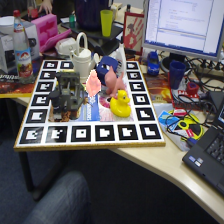
\includegraphics[width=0.9\textwidth]{figures/segmentation/ape_gt.png}
        \caption{Ape ground truth}
        \label{subfig:ape_ground_truth}
    \end{subfigure}
    \begin{subfigure}[t]{0.19\textwidth}
        \centering
        \captionsetup{width=.9\textwidth}
        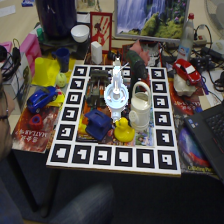
\includegraphics[width=0.9\textwidth]{figures/segmentation/bench_vise_gt.png}
        \caption{Bench vise ground truth}
        \label{subfig:bench_vise_ground_truth}
    \end{subfigure}
    \begin{subfigure}[t]{0.19\textwidth}
        \centering
        \captionsetup{width=.9\textwidth}
        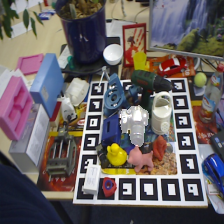
\includegraphics[width=0.9\textwidth]{figures/segmentation/cam_gt.png}
        \caption{Camera ground truth}
        \label{subfig:cam_ground_truth}
    \end{subfigure}
    \begin{subfigure}[t]{0.19\textwidth}
        \centering
        \captionsetup{width=.9\textwidth}
        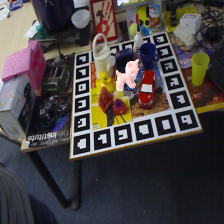
\includegraphics[width=0.9\textwidth]{figures/segmentation/cat_gt.png}
        \caption{Cat ground truth}
        \label{subfig:cat_ground_truth}
    \end{subfigure}
    \begin{subfigure}[t]{0.19\textwidth}
        \centering
        \captionsetup{width=.9\textwidth}
        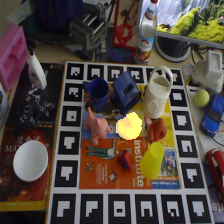
\includegraphics[width=0.9\textwidth]{figures/segmentation/duck_gt.png}
        \caption{Duck ground truth}
        \label{subfig:duck_ground_truth}
    \end{subfigure}

    \begin{subfigure}[t]{0.19\textwidth}
        \centering
        \captionsetup{width=.9\textwidth}
        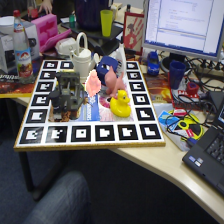
\includegraphics[width=0.9\textwidth]{figures/segmentation/ape_prediction.png}
        \caption{Ape prediction}
        \label{subfig:ape_prediction}
    \end{subfigure}
    \begin{subfigure}[t]{0.19\textwidth}
        \centering
        \captionsetup{width=.9\textwidth}
        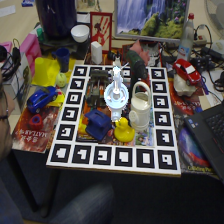
\includegraphics[width=0.9\textwidth]{figures/segmentation/bench_vise_prediction.png}
        \caption{Bench vise prediction}
        \label{subfig:bench_vise_prediction}
    \end{subfigure}
    \begin{subfigure}[t]{0.19\textwidth}
        \centering
        \captionsetup{width=.9\textwidth}
        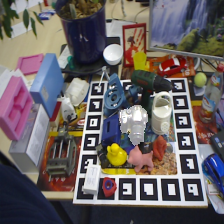
\includegraphics[width=0.9\textwidth]{figures/segmentation/cam_prediction.png}
        \caption{Camera prediction}
        \label{subfig:cam_prediction}
    \end{subfigure}
    \begin{subfigure}[t]{0.19\textwidth}
        \centering
        \captionsetup{width=.9\textwidth}
        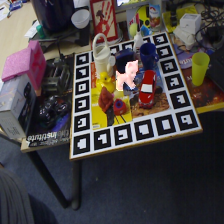
\includegraphics[width=0.9\textwidth]{figures/segmentation/cat_prediction.png}
        \caption{Cat prediction}
        \label{subfig:cat_prediction}
    \end{subfigure}
    \begin{subfigure}[t]{0.19\textwidth}
        \centering
        \captionsetup{width=.9\textwidth}
        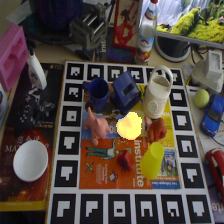
\includegraphics[width=0.9\textwidth]{figures/segmentation/duck_prediction.png}
        \caption{Duck prediction}
        \label{subfig:duck_prediction}
    \end{subfigure}
    \caption{Examples of semantic segmentation of the LINEMOD dataset. The first row contain the ground truth labels added to the input image, and the second row the corresponding predictions also added to the input image.}
    \label{fig:segmentation_example}
\end{figure}

The examples in figure \ref{fig:segmentation_example}, shows that the SegNet models detects each pixel of the object. The generated mask from the SegNet can now be used for feature extraction.

\subsubsection{Feature Extraction\\ \normalfont\normalsize\texttt{Mathias Emil Slettemark-Nielsen}} \label{subsubsec:feature_extration}
In DenseFusion the RGB input and depth input are processes separately to generate color and geometric features, because the RGB and depth information resides in different spaces. Therefore, two different network is implemented one for generate color embedding features and one for geometric embedding features.

\textbf{3D point cloud features:} The segmented depth pixels are converted into a 3D point cloud using the known camera intrinsics. The 3D point cloud is then fed to a geometric embedding network, that for each point generates a feature by mapping points to a $d_{geometric}$-dimensional feature space. This network is referred to as the geometric embedding network in figure \ref{fig:dense_fusion_overview}. The architecture is a multi-layer perceptron, MLP, followed by average pooling.

\textbf{Color image features:} To extract image features a CNN-based encoder-decoder architecture that maps an image of size $(H \times W \times 3)$ into $(H \times W \times d_{rgb})$ space is used. Thereby, making each pixel a $d_{rgb}$-dimensional vector that represents the input image pixel. This network is referred to as the image embedding network in figure \ref{fig:dense_fusion_overview}. The network consists of a ResNet-18 \cite{resnet} encoder followed by four upsampling layers as the decoder, the architecture of the network is illustrated in figure \ref{fig:image_embedding_network}.

\begin{figure}[H]
    \centering
    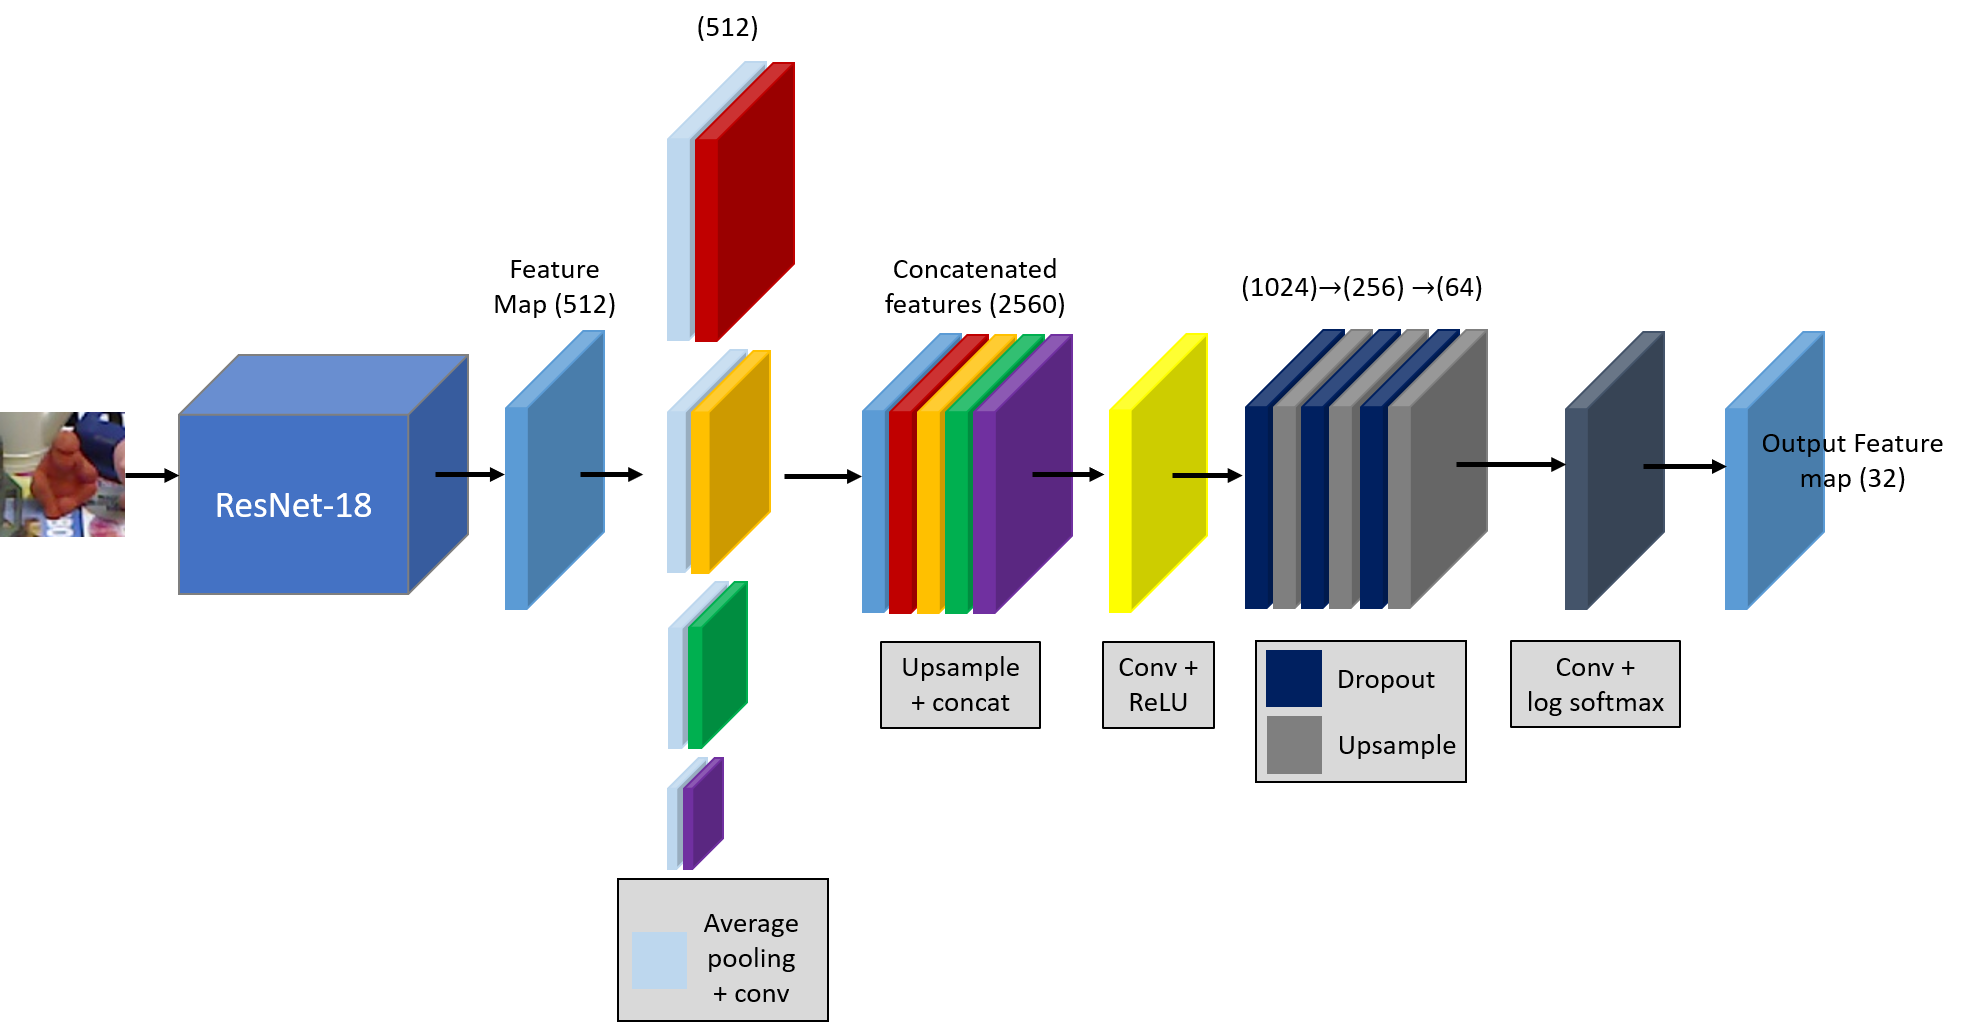
\includegraphics[width=\textwidth]{figures/dense_fusion/pspnet_architecture.png}
    \caption{An illustration of the image embedding network that encodes and decodes a image.}
    \label{fig:image_embedding_network}
\end{figure}

The image embedding network in figure \ref{fig:image_embedding_network} is inspired by Pyramid Scene Parsing Network, PSPNet, from \cite{pspnet}. PSPNet performs scene parsing based on semantic segmentation, thus it predicts the label, location and shape for each object. PSPNet introduces a pyramid pooling module that fuses features under four different scales, thereby making the detection more robust. The final output is a feature map that is passed on to the pose predictor network along with the gemometric featues as illustrated in figure \ref{fig:pixel_wise_fusion}.

\subsubsection{Pixel-wise Fusion for Pose Prediction\\ \normalfont\normalsize\texttt{Mathias Emil Slettemark-Nielsen}} \label{subsubsec:fusion}
The extracted features from the color image and 3D point cloud is now fused, thus each point contain information for each domain. DenseFusion performs local per-pixel fusion instead of global fusion so that predictions can be made based on each fused feature. 

The corresponding geometric feature and color feature are found based on a projection onto the image plane using the known camera intrinsic parameters. These features are then concatenated and used to generate a global feature, by a MLP followed by a averaging pooling. The fused feature is concatenated with the global feature and fed to a pose predictor network that predicts the 6D pose of the object, this process is illustrated in figure \ref{fig:pixel_wise_fusion}.

\begin{figure}[H]
    \centering
    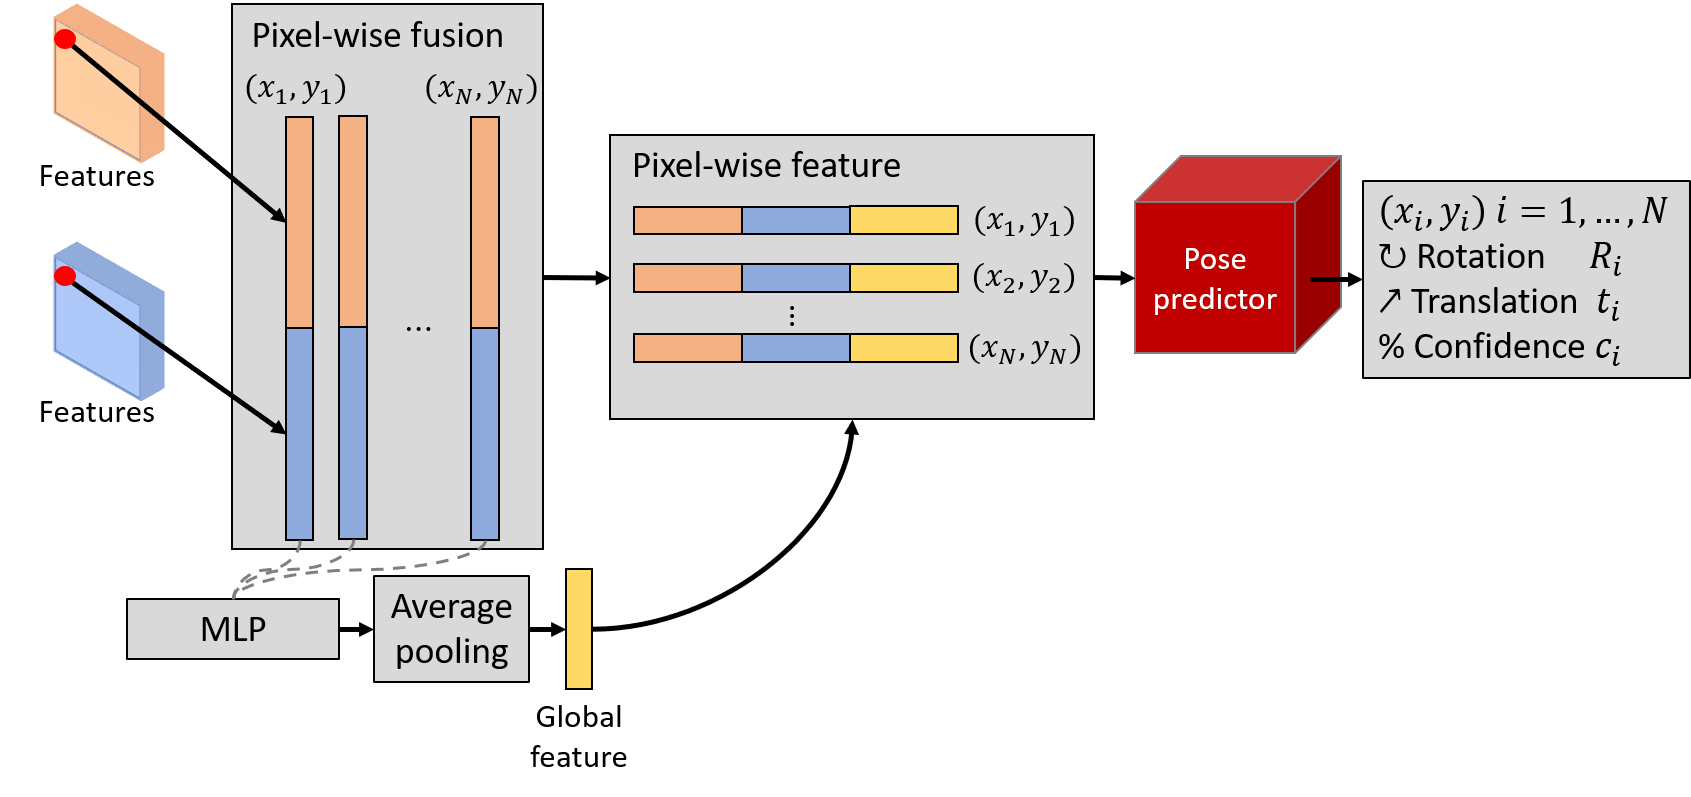
\includegraphics[width=\textwidth]{figures/dense_fusion/pixel_wise_fusion.png}
    \caption{An illustration of DenseFusion pose prediction where an estimated pose is generated for each pixel feature.}
    \label{fig:pixel_wise_fusion}
\end{figure}

The pose predictor network consists of three in parallel networks for rotation, translation and confidence. The networks consists of three MLP's with ReLU as activation function and a fourth MLP which differs for all three. The fourth MLP for the rotation has an output of four which represents a quaternion, likewise the fourth MLP for the translation has an output of three which represents the position in space. The fourth MLP for the confidence only has one output, the level of confidence for the estimated pose, and uses the sigmoid function as activation function.

The pose predictor network is trained to predict a pose to each fused feature. To decide the best estimated pose, the pose predictor outputs a confidence score $c_i$ for each pose estimation. This gives the pose predictor network two learning objective, pose estimation and confidence score. The pose estimation loss is the distance between the point from the ground truth pose and the corresponding point from the estimated pose. The pose estimation loss function to minimize is
\begin{equation}
    \label{eqn:loss_pose_estimation}
    L_i^p = \frac{1}{\mathcal{M}} \sum_{j=1}^{\mathcal{M}} \big\| (R x_j + T) - (\tilde{R_i} x_j + \tilde{t_i}) \big\|
\end{equation}
where $x_1$ is points of the objects 3D model $\mathcal{M}$, $p=[R | t]$ is the ground truth pose, and $\tilde{p_i}=[\tilde{R_i} | \tilde{t_i}]$ is the estimated pose generated from the fused feature of the $i$'th pixel. However, this loss function is only well defined for non-symmetric objects. Thus, for symmetric objects, the loss function finds the closest point between estimated model and the ground truth model. The loss function for symmetric objects is
\begin{equation}
    \label{eqn:loss_pose_estimation}
    L_i^p = \frac{1}{\mathcal{M}} \sum_{j=1}^{\mathcal{M}} \min_{k \in \mathcal{M}} \big\| (R x_j + T) - (\tilde{R_i} x_k + \tilde{t_i}) \big\|
\end{equation}
To learn the network to balance confidence among the predictions, the per pixel pose estimation loss is weighted with the corresponding confidence and a confidence regularization term is added. Thereby, the overall loss function is calculated as
\begin{equation}
    \label{eqn:loss_overall}
    L = \frac{1}{N} \sum_{i=1}^N \big( L_i^p c_i - w \log (c_i) \big)
\end{equation}
where $w$ is a balancing hyperparameter that is set to $0.015$ as in the paper \cite{densefusion}, and $N$ denotes the number of points randomly sampled from the segment. The pose estimation with the highest confidence is the final prediction as shown in figure \ref{fig:dense_fusion_overview}.

\subsubsection{Iterative Refinement\\ \normalfont\normalsize\texttt{Mathias Emil Slettemark-Nielsen}} \label{subsubsec:refinement}
DenseFusion uses an iterative refinement method to improve the predicted pose. This is done instead of using the Iterative Closest Point, ICP, algorithm \cite{icp}. The pipeline of the iterative refinement method is illustrated in figure \ref{fig:iterative_refinement}.

\begin{figure}[H]
    \centering
    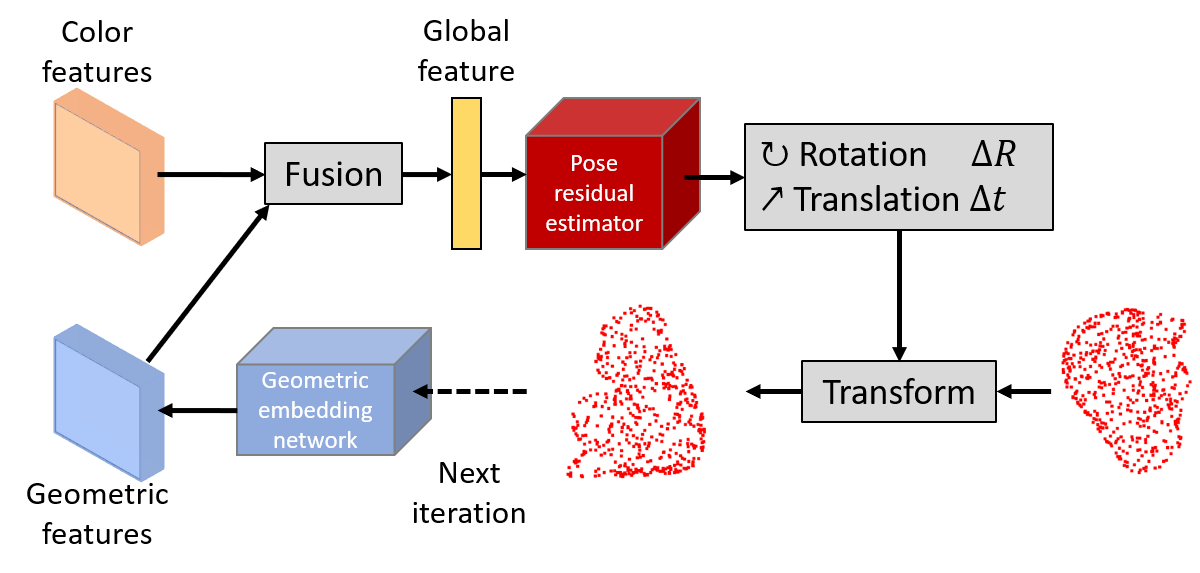
\includegraphics[width=\textwidth]{figures/dense_fusion/iterative_refinement.png}
    \caption{Iterative refinement of the predicted pose where a pose residual estimator predicts a residual pose.}
    \label{fig:iterative_refinement}
\end{figure}

The iterative refinement network takes the latest estimated pose and feeds it into the geometric embedding network. The color features and the new geometric features are fused to global features, which is fed to the pose residual estimator. The pose residual estimator predicts a residual pose based on the previously estimated pose and the generate global feature. After a number of iterations, $k$, the final pose estimation is obtained as
\begin{equation}
    \label{eqn:final_pose_estimation}
    \tilde{p} = [R_k | t_k] \cdot [R_{k-1} | t_{k-1}] \cdots [R_0 | t_0]
\end{equation}
The iterative refinement network consist of four fully connected layers that output the pose residual from the global feature, as illustrated in figure \ref{fig:iterative_refinement}. An illustration of the iterative refinement applied to a pose prediction is shown in figure \ref{fig:refinement_procedure}, where the reduction in the ADD score can be seen.

\begin{figure}[H]
    \centering
    \begin{subfigure}[t]{0.3\textwidth}
        \centering
        \captionsetup{width=.9\textwidth}
        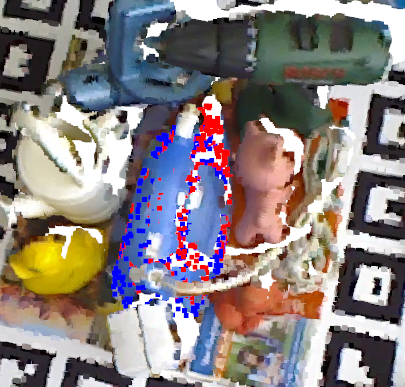
\includegraphics[height=40mm, keepaspectratio]{figures/dense_fusion/iron_refinement_0.png}
        \caption{ADD score: $0.0229$}
        \label{subfig:iron_refinement_0}
    \end{subfigure}
    \begin{subfigure}[t]{0.3\textwidth}
        \centering
        \captionsetup{width=.9\textwidth}
        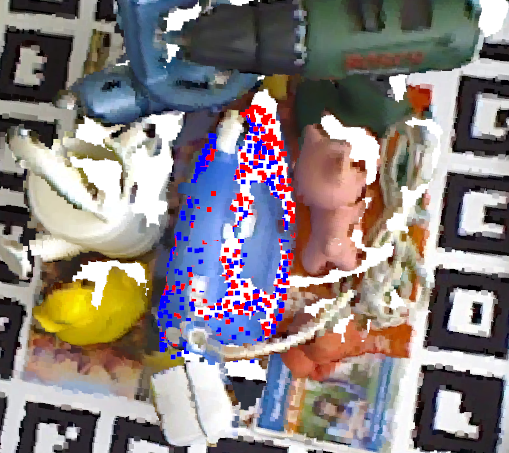
\includegraphics[height=40mm, keepaspectratio]{figures/dense_fusion/iron_refinement_1.png}
        \caption{ADD score: $0.0131$}
        \label{subfig:iron_refinement_1}
    \end{subfigure}
    \begin{subfigure}[t]{0.3\textwidth}
        \centering
        \captionsetup{width=.9\textwidth}
        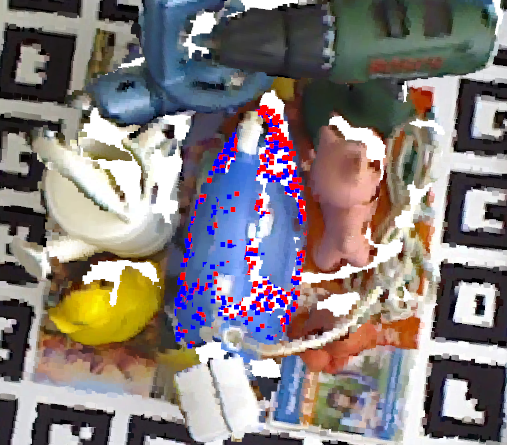
\includegraphics[height=40mm, keepaspectratio]{figures/dense_fusion/iron_refinement_2.png}
        \caption{ADD score: $0.00581$}
        \label{subfig:iron_refinement_2}
    \end{subfigure}
    \caption{Illustration of the iterative refinement procedure, where the estimate pose (blue points) and the ground truth pose (red points) is shown.}
    \label{fig:refinement_procedure}
\end{figure}

In figure \ref{fig:refinement_procedure}, it can be seen that the estimated pose, the blue points, gets closer to the ground truth pose, the red points, for each refinement iteration. This can also be seen by looking at the calculated ADD score that is descending. Further visualization of the iterative refinement procedure can be found at GitHub\footnote{\url{https://github.com/Masle16/obstacle_avoidance_with_dmps/blob/master/pose_estimation/dense_fusion/REFINENET.md}}.

\subsubsection{Implementation of Iterative Dense Fusion\\ \normalfont\normalsize\texttt{Mathias Emil Slettemark-Nielsen}} \label{subsubsec:imp_dense_fusion}
The LINEMOD dataset is split in approximately $15\ \%$ training and $85\ \%$ testing, as in the SegNet in section \ref{subsubsec:segnet}. The training set is repeated $20$ times before testing, and augmentation is added to the input image and the translation part of the 3D point cloud. The image augmentation is jittering in brightness, contrast, saturation and hue, and the 3D point cloud augmentation is random noise between $\pm0.03$.

In the paper \cite{densefusion}, they recommend to start the training of the iterative refinement network after the pose predictor has converged. Thus, the training is set to start when the pose predictor has a loss under $0.013$. The number of iterations, $k$, is set two $2$ as in the paper \cite{densefusion}. A learning rate of $0.0001$ is used with a decay of $0.3$, which is used when the network has a loss under $0.016$.

DenseFusion requires a lot of training and because of limited time and resources, the trained checkpoints from \cite{densefusion} is used as start parameters for the network.

\subsubsection{Evaluation of Iterative Dense Fusion\\ \normalfont\normalsize\texttt{Mathias Emil Slettemark-Nielsen}} \label{subsubsec:eval_dense_fusion}
Table \ref{tab:globpos:results} shows the results of the DenseFusion model on the LINEMOD dataset, and the evaluation as in \cite{linemod_matching_score} as described in section \ref{subsec:dataset} with the ADD/ADD-S metric. The prediction time of the DenseFusion method is $0.0259(\pm 0.0156)$ seconds. Visualization of the pose estimation by DenseFusion can be seen on GitHub\footnote{\url{https://github.com/Masle16/obstacle_avoidance_with_dmps/blob/master/pose_estimation/dense_fusion/RESULTS.md}}.

To evaluate the robustness of the DenseFusion model noise is added to the input, both the RGB image and the 3D point cloud. The noise added is sampled from a normal distribution with zero mean and varying standard deviation, and the noise added to the RGB image is scaled with the maximum pixel value $255$. The noise experiments can be seen in figure \ref{fig:noise_experiments}.
\begin{figure}[H]
    \centering
    \begin{subfigure}[t]{0.49\textwidth}
        \centering
        \captionsetup{width=.9\textwidth}
        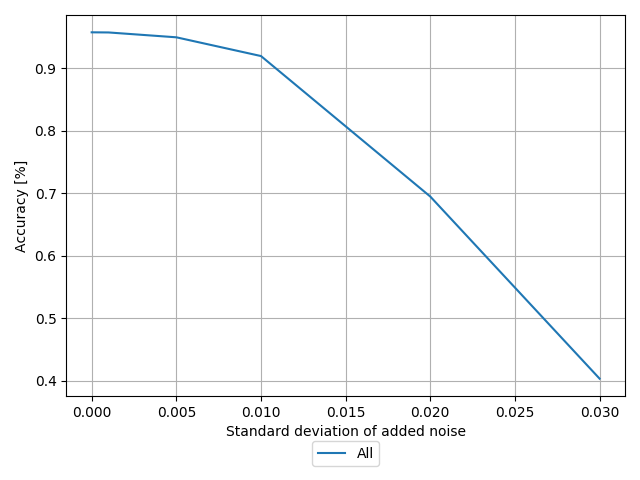
\includegraphics[width=\textwidth]{figures/dense_fusion/acc_all.png}
        \caption{The overall accuracy when noise is added to the input.}
        \label{subfig:noise_all}
    \end{subfigure}
    \begin{subfigure}[t]{0.49\textwidth}
        \centering
        \captionsetup{width=\textwidth}
        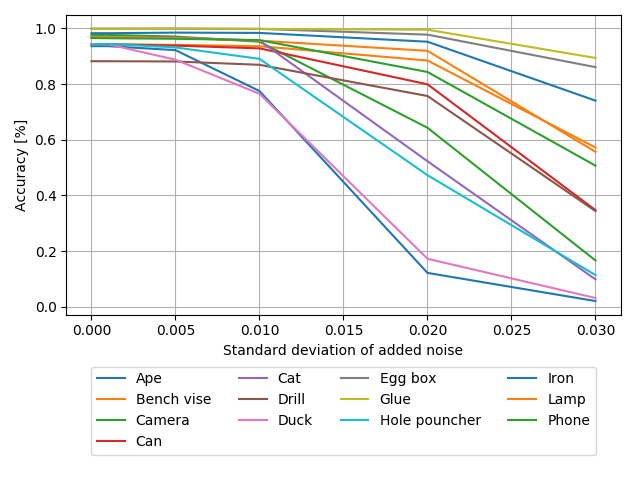
\includegraphics[width=\textwidth]{figures/dense_fusion/acc_objs.png}
        \caption{Accuracy of each object when noise is added to the input.}
        \label{subfig:noise_objects}
    \end{subfigure}
    \caption{Noise experiments of DenseFusion.}
    \label{fig:noise_experiments}
\end{figure}

From figure \ref{subfig:noise_all}, the overall accuracy of DenseFusion drops below $50\ \%$ when noise with a standard deviation of $0.03$ is applied. However, when looking at the individual objects in \ref{subfig:noise_objects} some objects still have a accuracy above $50\ \%$. The object Ape and Cat drops below $50\ \%$ at a standard deviation of $0.015$. The performance of DenseFusion is deemed acceptable until a standard deviation of $0.01$ where the overall accuracy is $91.98\ \%$, and the lowest individual accuracy is $77.5\ \%$.

\subsection{3D - 3D Pose Estimation\\ \normalfont\normalsize\texttt{Mikkel Larsen}} \label{subsec:3d-3d}
In order to compare the performance of the 6D pose estimation of the DenseFusion network a baseline method is chosen. The method is a traditional pose estimation method consisting first of a global pose alignment followed by a local pose alignment. The input to the method is a 3D model of the object and a 3D scene where the object has been segmented. Both the 3D model and scene is a point cloud. The 3D segmented object is generated by the SegNet as described in \autoref{subsubsec:segnet}. The implemented global alignment and local alignment method used is from the library open3d \cite{open3d}.

\subsubsection{Alignment Parameter Choice}
The global alignment is a RANSAC algorithm using both a point cloud of the model and the segmented object and corresponding point cloud feature descriptors. The implemented global alignment method uses Fast Point Feature Histogram, FPFH, as a descriptor. The FPFH uses surface normal for each point to construct a k-d tree in order to related the points to each other. Here the radius for the surface normal is set to $0.25$ and the maximum number of neighbor points to $15$. The k-d tree parameters are set to a radius feature of $0.5$ and maximum number of neighbor point of $30$.

The RANdom SAmple Consensus algorithm, RANSAC, saves the best transformation based on point inliers from model point cloud to segmented point cloud. The distance threshold between points from the model and segmented is set to $0.1$. The same distance is also used when specifying the maximum distance between feature point pairs. Furthermore, the maximum number of iterations of RANSAC is either $4\cdot10^5$ or $10^4$ new best transformations. Using $10^4$ yielded significant better accuracy but also longer evalution time as shown in \autoref{tab:globpos:val:perf}. 

The local alignment method uses Iterative Closest Point, ICP. The same distance threshold between points from the model point cloud and the segmented point cloud of $0.1$ is used. 

\subsubsection{Evaluation of 3D - 3D Pose Estimation}
A test to decide the maximum number of validation were conducted. Because of time constraint the test were only conducted on the first 10 objects of each class of the LINEMOD dataset. The results is listed in \autoref{tab:globpos:val:perf}.
\begin{table}[H]
\centering
\begin{tabular}{l|llll}
\toprule
\textbf{Max number of validations} & $10^4$ & $10^3$ & $10^2$ & $10$ \\ \hline
\textbf{Total Accuracy [\%]} & $62.3$ & $47.7$ & $22.3$ & $19.2$ \\ \hline
\textbf{Iterations pr time [it/s]} & $0.58$ & $3.77$ & $7.83$ & $8.95$ \\ \bottomrule
\end{tabular}
\caption{Test of max number of validation of RANSAC in 3D-3D pose alignment, logging time and accuracy. Tested with all object classes but only for the first 10 objects.  }
\label{tab:globpos:val:perf}
\end{table}

The same evaluation is done for 3D-3D pose estimation as for DenseFusion described in \autoref{subsubsec:eval_dense_fusion} on the LINEMOD dataset. The results is shown in \autoref{tab:globpos:results}.

\begin{table}[H]
\centering
\resizebox{\textwidth}{!}{%
\begin{tabular}{@{}l|ll|ll@{}}
\toprule
& \multicolumn{2}{c|}{\textbf{DenseFusion}} & \multicolumn{2}{c}{\textbf{3D - 3D}} \\
& Accuracy [\%] & ADD/ADD-S [cm] & Accuracy [\%] & ADD/ADD-S [cm] \\ \midrule
\textbf{Ape} & $93.71$ & $0.005(\pm 0.00603)$ & $51.38$ & $0.02457(\pm 0.02217)$ \\
\textbf{Bench vise} & $94.67$ & $0.00767(\pm 0.0146)$ & $59.94$ & $0.03895(\pm 0.04337)$ \\
\textbf{Can} & $97.45$ & $0.00638 (\pm 0.00928)$ & $44.61$ & $0.04761 (\pm 0.04139)$ \\
\textbf{Camera} & $94.69$ & $0.00675(\pm 0.0143)$ & $52.17$ & $0.04602(\pm 0.04364)$ \\
\textbf{Cat} & $96.71$ & $0.00468(\pm 0.00852)$ & $57.78$ & $0.02940(\pm 0.03124)$ \\
\textbf{Drill} & $88.31$ & $0.0143(\pm 0.0263)$ & $65.01$ & $0.03546(\pm 0.04351)$ \\
\textbf{Duck} & $93.90$ & $0.00629(\pm 0.0191)$ & $46.49$ & $0.02989(\pm 0.03083)$ \\
\textbf{Eggbox} & $99.81$ & $0.00763(\pm 0.0011)$ & $99.81$ & $0.00744(\pm 0.002588)$ \\
\textbf{Glue} & $99.81$ & $0.00481(\pm 0.00192)$ & $99.90$ & $0.00611(\pm 0.002708)$ \\
\textbf{Hole pouncher} & $94.01$ & $0.00683(\pm 0.0102)$ & $37.68$ & $0.04104(\pm 0.03168)$ \\
\textbf{Iron} & $98.47$ & $0.00651(\pm 0.0111)$ & $41.47$ & $0.07298(\pm 0.05758)$ \\
\textbf{Lamp} & $97.02$ & $0.00638(\pm 0.0143)$ & $66.41$ & $0.03337(\pm 0.04200)$ \\
\textbf{Phone} & $96.35$ & $0.00693(\pm 0.0121)$ & $73.97$ & $0.02137(\pm 0.02907)$ \\ \midrule
\textbf{All} & $95.76$ & $0.00693(\pm 0.0133)$ & $61.28$ & $0.03510(\pm 0.03240)$ \\ \bottomrule
\end{tabular}%
}
\caption{Result of the implemented DenseFusion and 3D-3D pose estimation methods on the LINEMOD dataset.}
\label{tab:globpos:results}
\end{table}

From table \ref{tab:globpos:results}, the method DenseFusion scores a overall accuracy of $95.76\ \%$ whereas the 3D-3D gets $61.28\ \%$. The 3D-3D method only gets a better accuracy with the glue object. However, there is only a difference between the two methods of $0.09$. The prediction time of DenseFusion is $0.0259$ seconds and 3D-3D is $1.72$ seconds, thus DenseFusion predicts significantly faster than the 3D-3D method. 
 
\end{document}